\chapter{Analysis of existing corporation}

As an example of an existing service implementation let's take an anonymous company. For the purpose of this thesis it will be named Invest s.r.o.. The company is operating on the market more than ten years and during this period was reorganised to service-oriented architecture. Invest s.r.o. has many clients in its portfolio. Many of them are consuming services provided by this company.

\section{Architecture overview}
Architecture of Invest s.r.o. can be divided into multiple layers. In sake of providing services to the third party the application is composed by Data layer, Application layer, Integration layer as is shown on Figure \ref{fig:invest-architecture}.

\begin{figure}[htp] \centering{
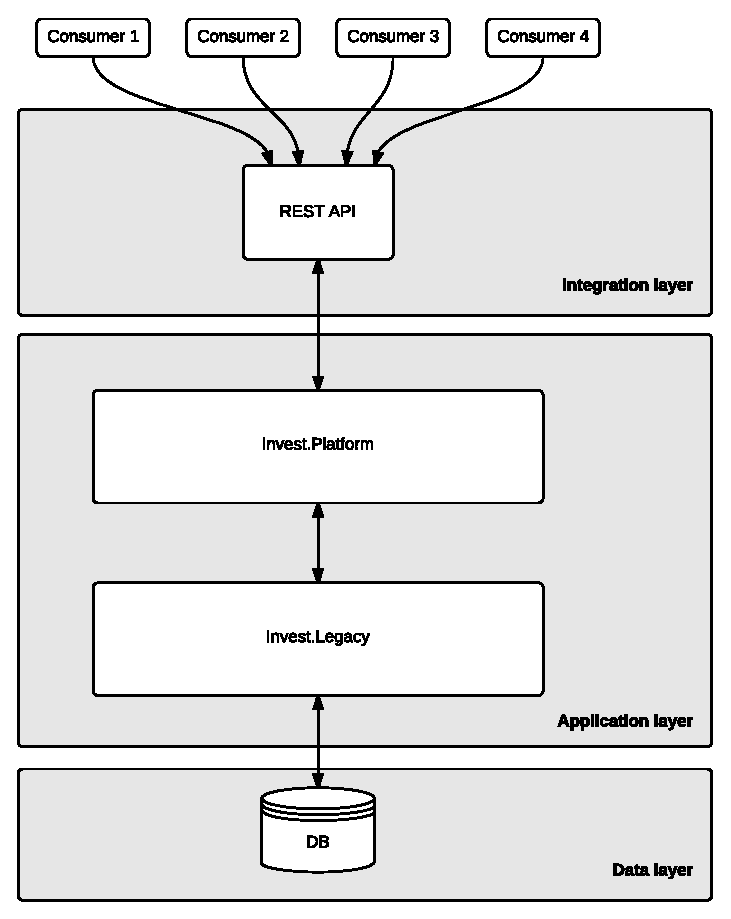
\includegraphics[width=8cm]{img/invest-architecture.pdf}}
\caption{Invest s.r.o. architecture}
\label{fig:invest-architecture}
\end{figure} 

The highest layer of application is than Integration layer containing service API. It provides access points for integration of services. The Application layer holds the whole business logic. Every logical functionality is performed in this layer. Every data are stored within Data layer.

\section{Integration layer}
Services present on the Integration layer are REST-based. They are designed in REST style but it wasn't suitable to make them RESTful. Services are providing to third party connection on the functionality and data present in underlying layers.

